%{{{ Preamble
\documentclass[usenatbib]{mnras}
\usepackage{graphicx}
\usepackage[export]{adjustbox}
\usepackage{bm}
\usepackage{amsmath}
\usepackage{amssymb}
\usepackage{algorithm}
\usepackage{algpseudocode}
\usepackage{subcaption}
\usepackage{layouts}
\usepackage{hyperref}
\usepackage[capitalise]{cleveref}
\usepackage{fancyvrb}
\usepackage{xcolor}
\usepackage{txfonts}
\usepackage[T1]{fontenc}
%}}}

%{{{ Commands
\newcommand{\logL}{\{ \log \Like_i \}}
\newcommand{\thetab}{\bm{\theta}}
\newcommand{\logLm}{\log \Like_\mathrm{max}}
\newcommand{\set}[1]{\{#1\}}
\newcommand{\nlive}{n_\mathrm{live}}
\newcommand{\Like}{\mathcal{L}}
\newcommand{\DKL}{\mathcal{D}_\mathrm{KL}}
%}}}

\title[Approximating the end of nested sampling]{Approximating the end of nested sampling}
\author[Z. Hu et. al]{Zixiao Hu, Artyom Baryshnikov, Will Handley}


\begin{document}
\label{firstpage}
\pagerange{\pageref{firstpage}--\pageref{lastpage}}
\maketitle


\begin{abstract}
This paper develops a technique to estimate the runtime of a nested sampling run at an intermediate iteration which works for any nested sampling implementation. The known likelihood at an iteration is fitted, then extrapolated using a Gaussian model function, which allows the remaining evidence and prior volume at termination to be calculated. We find that the method succesfully recovers the true endpoint within standard error from the beginning for near-Gaussian likelihoods. For non-Gaussian likelihoods, the estimate is still the correct order of magnitude and converges to the correct answer by the end of the run.
\end{abstract}

\begin{keywords}
methods: data analysis -- methods: statistical
\end{keywords}

\section{Introduction}
Nested sampling is a multi-purpose algorithm invented by John Skilling which simultaneously accomplishes the two tasks of Bayesian inference, model comparison and parameter estimation \citep{skilling}. It was immediately adopted for cosmology, and is now used in a wide range of physical sciences including particle physics, materials science \citep{physical_scientists} and machine learning \citep{sparse_reconstruction}. The core algorithm is unique for estimating volumes using \textit{order statistics}, which makes high-dimensional integration feasible. It also avoids problems faced by traditional Bayesian algorithms, such as multi-modality.
\par
Many instances of software for nested sampling exist, including popular implementations such as \textsc{MultiNest} \citep{multinest} and \textsc{PolyChord} \citep{polychord}, as well as post-processing packages such as \textsc{anesthetic} \citep{anesthetic} to plot sample statistics and distributions. However, no such software is currently able to estimate how long a given run should last. This is of high importance to the end user, who has no indication in the middle of a run whether it will take hours, or weeks and months to finish; even an order of magnitude estimate is useful compared to the status quo of complete ignorance.
\par
This project sets out a novel approach for estimating the endpoint of a nested sampling run at an intermediate stage, an example of which is shown in \cref{fig:polychord_output}. The idea is to predict the form of the likelihood function in the region we have yet to sample from, using the information we have already gained from our previous samples. We begin in section \cref{sec:Background} with an overview of nested sampling, before discussing its convergence properties in \cref{sec:convergence}. \cref{sec:method} presents the methodology of making endpoint predictions, before results for both toy and real examples are shown in section \cref{sec:results}. Finally, conclusions are made in section \cref{sec:conclusions}.
\par
Users would like a order of magnitude runtime estimate
\begin{figure}
\begin{Verbatim}[frame=single, commandchars=\\\{\}]
\textcolor{red}{Predicted endpoint: 25054 +/- 242}
\textcolor{red}{Progress: [=================>########] 72%}
___________________
lives      |   500 |
phantoms   | 24310 |
posteriors | 18018 |
equals     |   245 |
-------------------
ncluster   =  1/1
ndead      =  18018
nposterior =  18018
nequals    =  249
nlike      =  4159049
<nlike>    =  491.04 (9.82 per slice)
log(Z)     =  -12.55 +/- 0.27
\end{Verbatim}
\caption{Output from \textsc{PolyChord} for a typical nested sampling run. The predicted endpoint, shown in red, is calculated using the method described in this paper.}
\label{fig:polychord_output}
\end{figure}
\section{Background}\label{sec:Background}
Let us begin with a brief description of the nested sampling algorithm and several adjacent concepts to establish the necessary notation. 
\subsection{Nested sampling}
For a given likelihood $\mathcal{L}(\theta)$ and prior $\pi(\theta)$, nested sampling simultaneously calculates the Bayesian evidence
\begin{equation}\label{eq:evidence}
	\mathcal{Z} = \int \mathcal{L}(\theta)\ \pi(\theta)\ \mathrm{d}\theta
\end{equation}
while producing samples of the posterior distribution
\begin{equation}
	\mathcal{P}(\theta) = \frac{\mathcal{L}(\theta) \pi(\theta)}{\mathcal{Z}}.
\end{equation}
The algorithm operates by maintaining a set of $\nlive$ \textit{live points} sampled from the prior, which can vary in number throughout the run. At each iteration, the point with the lowest likelihood is removed and added to a list of \textit{dead points}. A new point is then drawn from the prior, subject to the constraint that it must have a higher likelihood than the latest dead point. Repeating the procedure leads to the live points shrinking around peaks in the likelihood.
\par
The integral in \cref{eq:evidence} is then evaluated by transformation to a one-dimensional integral over the \textit{prior volume} $X$, defined as
\begin{equation}
	\mathcal{Z} = \int_0^1 \mathcal{L}(X)\ \mathrm{d}X \approx \frac{1}{2}\sum_{i=1} \mathcal{L}(X_{i-1}-X_{i+1}),
\end{equation}
where $X(\mathcal{L})$ is the fraction of the prior greater than $\mathcal{L}$. The prior volumes $X_i$ are unknown, but can be statistically estimated as follows: one can define a \textit{shrinkage factor} $t_i$ at each iteration $X_{i} = t_i X_{i-1}$, such that
\begin{equation}\label{eq:X_dist}
	X_i = \prod_{k=1}^i t_k.
\end{equation}
The $t_i$ are the maximum of $\nlive$ points drawn from $[0,1]$, so follow the distribution
\begin{equation}\label{eq:t_dist}
	P(t_i) = \nlive t_i^{\nlive-1}, \quad \langle\log t_i\rangle = -\frac{1}{\nlive}, \quad \mathrm{Var}(\log t_i) = \frac{1}{\nlive^2}.
\end{equation}
The algorithm terminates when an user-specified condition is met; a popular choice is to terminate when the evidence in the live points falls below some fraction $\epsilon$ of the accumulated evidence e.g. $10^{-3}$. The remaining live points are then killed off one by one without replacement and added to the evidence.
\par
Uncertainties in the evidence are dominated by the spread in the prior volume distribution, and the simplest way to estimate them is by Monte Carlo sampling over sets of $\bm{t}$.
\par
The time complexity of nested sampling, as analysed in \citet{supernest}, is
\begin{equation}
    T \propto \nlive \times \langle \mathcal{T}\{ \Like(\theta) \} \rangle \times \langle \mathcal{T}\{ \mathrm{Impl.}\} \rangle \times \mathcal{D}_\pi \{ \mathcal{P} \}.
\end{equation}
For a given resolution of $\nlive$, the runtime is therefore proportional to the average time for a likelihood evaluation, the implementation-dependent average time to sample a higher likelihood live point, and the information gain from prior to posterior. The first two of these are typically constant over the course of a run, so the runtime is primarily determined by the compression factor $\mathcal{D}$.

\subsection{Thermodynamic connection}\label{sec:thermodynamic}
The thermodynamic generalisation of Bayes' theorem is given by
\begin{equation}\label{eq:thermo_bayes}
    \mathcal{P}_\beta(\theta) = \frac{\mathcal{L}^{\beta}(\theta) \pi(\theta)}{\mathcal{Z}(\beta)},
    \quad
    \mathcal{Z}(\beta) = \int \mathcal{L}(\theta)^\beta \pi(\theta)\ \mathrm{d}\theta,
\end{equation}
where $\beta$ is the inverse temperature $1/T$. If each $\theta$ is a microstate, then $\log \mathcal{L}$ becomes the negative energy, $\pi$ becomes the density of states, and $\mathcal{Z}$ naturally the partition function. The advantage of nested sampling for computing partition functions is that it compresses at a constant thermodynamic speed by taking samples equally spaced in volume entropy, which sidesteps the problem of designing an annealing schedule \citep{statmech}.  

\subsection{Bayesian model dimensionality}\label{sec:dimensionality}
Following the thermodynamic connection, an important construct is the analogue of the heat capacity, which is the \textit{Bayesian model dimensionality}, defined as the posterior variance of the Shannon information: 
\begin{equation}
\frac{\tilde{d}}{2} = \int \mathcal{P}(\theta) \left(\log \frac{\mathcal{P}(\theta)}{\pi(\theta)} - \DKL\right)^2 \: \mathrm{d}\theta
= \langle \mathcal{I}^2 \rangle_\mathcal{P} - \langle \mathcal{I} \rangle^2_\mathcal{P}.
\end{equation}
Just as the heat capacity is a measure of the number of degrees of freedom in a system, the Bayesian model dimensionality is a measure of the number of constrained parameters in a set of samples.

\section{The progress of a nested sampling run}\label{sec:convergence}
We will now present several useful ways of measuring the progress of a nested sampling run, together with an assortment of results we shall use to make endpoint predictions. At a given iteration $i^{*}$, these are the current prior volume $\log X^{*}$ of the latest dead point, the corresponding log-likelihood $\log\Like^{*}$, and the current effective temperature $\beta^{*}$ of the samples. 
\subsection{Current prior volume}\label{sec:volume_convergence}
The conventional perspective for the progress of a run is with $\log X$ along the x-axis, where the prior volume is compressed at a steady rate until we reach the posterior mass. Defining the Kullback-Leibler divergence as
\begin{equation}\label{eq:DKL}
	\DKL = \int \mathcal{P}(\theta) \log \frac{\mathcal{P}(\theta)}{\pi(\theta)}\ \mathrm{d}\theta,
\end{equation}
we interpret it as the posterior averaged logarithmic \textit{volume compression} from the prior to the posterior. Hence we can define a  \textit{posterior bulk} at below $X = e^{-\DKL}$ containing nearly all of the information, which gives us a measure of the volume we must compress down for the algorithm to converge.
\par
At an intermediate iteration $i_*$, we only have samples of the posterior only down to the current prior volume $\log X_*$. We do have some information below this volume due to the live points, but we will see now that they do not bring us much further. If we kill off all the live points as if we were terminating, then by \cref{eq:t_dist} the prior volume of the final live point $\log X_\mathrm{min}^{\mathrm{live}}$ has mean and variance given by
\begin{equation}
	\mathrm{E}[\log X_\mathrm{min}^{\mathrm{live}}] = \mathrm{E}[\log X_*] - \sum_{k=1}^{\nlive} \frac{1}{n_k} \approx -\frac{i_*}{\nlive} - \log \nlive - \gamma,
\end{equation}
\begin{equation}
	\mathrm{Var}[\log X_\mathrm{min}^{\mathrm{live}}] = \mathrm{Var}[\log X_*] + \sum_{k=1}^{\nlive} \frac{1}{n_k^2} \approx \frac{i_*}{\nlive^2} + \frac{\pi^2}{6},
\end{equation}
where the large $\nlive$ limit is taken for the approximation to the harmonic series, $\gamma$ being the Euler-Mascheroni constant.
\par
This shows that the live points only get us a factor of $\log \nlive$ closer to the posterior bulk. In other words, it is not until we are around $\log \nlive$ away from $\log X = \DKL$ that the samples look anything like the posterior. One can see from \cref{eq:DKL} that the divergence increases linearly with dimension, so for large dimensionalities (such as the Planck legacy chains, which have a $\DKL$ of $\sim 40$) and typical live point numbers of  $\sim 1000$, this does not happen until near the end of the run.
\par
Intuitively, this is because for a sharply peaked likelihood the live points are too diffuse to land there with any significant probability for most of the run.
\begin{figure*}
\begin{center}
	\includegraphics{figures/live_point_distribution.pdf}
\end{center}
\caption{The distribution of the posterior mass in terms of $\log X$, the live points over the prior $\pi(\log X \mid \log X < \log X_*)$ and the smallest live point prior volume $\log X_\mathrm{min}^{\mathrm{live}}$ at an intermediate iteration $i_*$. For large values of $\DKL$ i.e. informative posteriors and/or large dimensionalities, the maximum live point is very far from the posterior bulk until the very end of the run. Note that the x-axis in this plot is $\log X$, so that the run proceeds from right to left to emphasise that the enclosed prior volume iteratively gets smaller. Plots of the sort from here onwards will be in terms of $-\log X$, where the run will more naturally proceed from rleft to right. }
\label{fig:live_point_distribution}
\end{figure*}

\subsection{Current log-likelihood}
We can also view the run as a function of the current log-likelihood value $\log\mathcal{L}^{*}$, which of course monotonically increases throughout the run. To illustrate some of the analytics, let us take the example of a Gaussian likelihood with dimension $d$ and lengthscale $\sigma$;
\begin{equation}\label{eq:logL}
	\log\mathcal{L} = \log\mathcal{L}_\mathrm{max} - \frac{X^{2/d}}{2\sigma^2}.
\end{equation}
$\log \mathcal{L}^{*}$ must increase until the posterior bulk is passed, which is located around the posterior averaged log-likelihood 
\begin{equation}
    \langle\log\mathcal{L}\rangle_\mathcal{P} = \log\mathcal{L}_\mathrm{max} - \frac{d}{2},  \quad \mathrm{Var}(\log\mathcal{L})_\mathcal{P} = \frac{d}{2}.
\end{equation}
Given the value of the latest dead point, we can examine the distribution of the live points in likelihood. Define the normalised likelihood
\begin{equation}
    y = \frac{\log\mathcal{L}-\log\mathcal{L}_*}{\log\mathcal{L}_\mathrm{max}-\log\mathcal{L}_*}
    \label{eq:normalised_likelihood}
\end{equation}
as a measure of how far a point is between the current likelihood and the maximum; $y=0$ corresponds to $\log\mathcal{L}_*$ and $y=1$ to $\log\mathcal{L}_\mathrm{max}$. It follows that the live points are distributed as 
\begin{equation}
    P(y) = \frac{d}{2}(1-y)^{\frac{d}{2}-1} \quad [0<y<1],
    \label{eq:Py}
\end{equation}
and the maximum live point has mean and variance
\begin{equation}\label{eq:ylivemax}
	\lim_{d,\nlive\to\infty} y_\mathrm{max}^\mathrm{live} \sim \frac{2\log \nlive}{d} \pm \sqrt{\frac{2}{3}}\frac{\pi}{d}
\end{equation}
in the limit of large $d$ and $\nlive$ (see appendix for derivation). We therefore see that just as with the prior volumes, in high dimensions the live points only bring us logarithmically further, while $d$ pushes us linearly away.

\subsubsection*{Nested sampling as a maximiser}
Previous literature has explored the potential of nested sampling algorithms as maximisers \citep{Akrami_2010, Feroz_2011}. The latter authors emphasised the terminatioin criterion controls the global maximum obtained. 
\par
We can use these results to show that nested sampling by itself is a poor maximiser. If we set $\log\Like^{*}$ to be the termination point $\log\Like_\mathrm{end}$, we can invert \cref{eq:normalised_likelihood} to find that the maximum live point is located at
\begin{equation}
    \boxed{
        \log{\mathcal{L}}_\mathrm{max}^\mathrm{live} \approx \log\mathcal{L}_\mathrm{max} - \frac{d}{2e} + \frac{\log n}{e} \pm \frac{\pi}{\sqrt{6}e}
    }.
\end{equation}
Hence in general nested sampling will finish at a contour $d/2e$ away from the maximum log-likelihood, and the final set of $n$ live points can get you $(\log n)/2e$ closer, with a chance of getting $\sim\pi/\sqrt{6}e=0.472$ closer still by statistical fluctuation. 
\par
We find that in higher dimensions (typically greater than ten), the maximum live point is nowhere near the true maximum! However, these shortcomings can be mitigated by using the maximum point in the chain as a \textit{starting point} for a gradient-based optimisation algorithm, which would allow us to leverage the advantages of nested sampling to navigate multimodal landscapes while also rapidly approach the maximum point.
\begin{figure*}
\begin{center}
	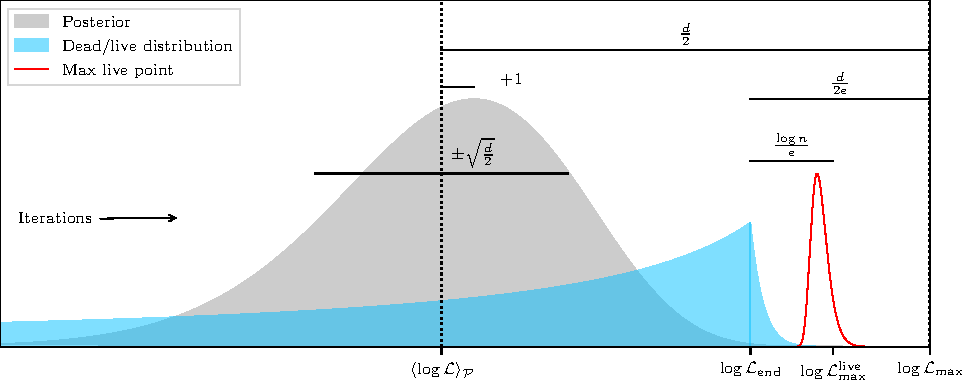
\includegraphics{figures/anatomy.pdf}
\end{center}
\caption{Distribution of samples as a function of $\log\mathcal{L}$, showing the posterior $\mathcal{P}(\log\mathcal{L})$, the distribution of the live points $\mathcal{\pi}(\log\mathcal{L} \mid \mathcal{L}>\mathcal{L}_*)$, and the distribution of the maximum likelihood live point $P(\log\mathcal{L}_\mathrm{max}^\mathrm{live})$}
\label{fig:anatomy}
\end{figure*}

\subsection{Current temperature}\label{sec:current_temperature}
As previously discussed, nested sampling chooses an annealing schedule that moves at constant thermodynamic speed, which constructs a gradual transition from prior ($\beta = 0$) to posterior ($\beta = 1$). One can expect then that any given point during a run can be associated with a $\beta \in [0,1]$ that measures how far the current set of samples lies between prior and posterior. 
\par
We present here the idea that one can assign each iteration of a nested sampling run $i^{*}$ with a \textit{current temperature} $\beta^*$.
\par
As noted by Skilling, the posterior with respect to $\log X$ $\Like^{\beta} X$ has a peak at $\log X^*$ when  
\begin{equation}
    \beta^* = - \frac{\mathrm{d} \log X}{\mathrm{d} \log \Like}
\end{equation}



\subsubsection*{Choice of temperature mapping}
The typical behaviour at an intermediate stage of a nested sampling run is that the posterior mass is dominated by a single point. This is because the highest live point is typically several log-likelihoods, and therefore orders of magnitude higher in weight than the next point. Decreasing $\beta$, equivalent to increasing the temperature, causes the mass to redistribute more equally across the samples. A natural choice for the present temperature $\beta^{*}$ is therefore one where the posterior mass is concentrated around the current dead point. What that constitutes is subjective, and several plausible choices are presented below:
\begin{itemize}
    \item Setting the posterior averaged log-likelihood $\langle \log\Like \rangle_{\mathcal{P}(\beta)}$ to be equal to the current $\log\Like^{*}$.
    \item Setting the Kullback-Leibler divergence of current set of samples $\mathcal{D}(\beta)$ to be equal to the current $-\log X^{*}$.
    \item Setting $\beta$ so that the set of samples meets some criterion for the remaining posterior mass, for example so that a specified fraction $\epsilon$ of the total mass lies beyond the current point.
\end{itemize}
Note that the second condition is a special case of the third, since $\DKL = \langle \log\Like \rangle_\mathcal{P} - \log \mathcal{Z} = -\log X^{*}$ corresponds to $\mathcal{Z} \sim \mathcal{L}X$ so that $\epsilon \sim 0.5$. One could account for the uncertainty in choice by sampling uniformly between the $\beta^{*}$ that correspond to fractions $\epsilon$ and $1 - \epsilon$ of the posterior mass remaining, since all such choices have a posterior mass 
\par

\subsubsection*{Inferring the current temperature}
Transforming $\mathcal{L} \to \Like^{\beta}$ leads to the posterior distribution for $\log X$ to instead follow
\begin{equation}
    \mathcal{P}\left(\log X \mid \beta\right) = \frac{\Like^{\beta} X}{\int \Like^{\beta} X \ \mathrm{d}\log X}.
\end{equation}
Using Bayes' rule one can get reverse, which is the probability of the temperature given a set of $\log X$;
\begin{equation}
    P\left(\beta \mid \log X\right) \propto \mathcal{P}\left(\log X \mid \beta\right)P\left(\beta\right).
\end{equation}
Evaluating the left hand side for $\log X = \log X^{*}$ then gives the distribution of $\beta$ at the current iteration. We note that we would like $P\left(\beta = 0 \mid \log X^{*}\right) = 0$ since the likelihood must always increase, but $\Like^{\beta} X^{*} = X^{}$  


\subsubsection*{Intermediate sample dimensionalities}
One problem with the Bayesian model dimensionality is that it is practically zero for most of the run, only converging at the very end when the posterior mass is no longer concentrated at a single point with zero variance. From the thermodynamic perspective, this is expected; the present number of degrees of freedom only corresponds to the heat capacity at the present, not the final temperature. The number of parameters constrained at an intermediate stage should really be calculated from the \textit{transformed} posterior, not the original set of samples.
\par
Plotted below are the temperature adjusted sample dimensionalities for a spherical Gaussian, for which the ground truth is known. 

\begin{figure}
\begin{center}
	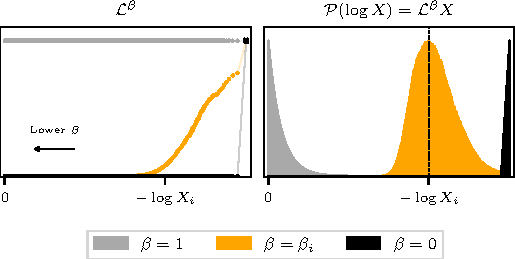
\includegraphics{figures/last_live_point.pdf}
\end{center}
\caption{The likelihood profile and posterior mass as $\beta$ is lowered. The original likelihood is shown in black, which is dominated by the maximum live point. As $\beta$ decreases, the posterior mass is shifted back from the maximum point to the other points, until so much of the mass has shifted that the present point $\log X^{*}$ is the termination point. The transformed likelihood and posterior at this point is shown in orange.}
\label{fig:last_live_point}
\end{figure}

If this quantity is computed from the untransformed samples, it will output zero since there is effectively only one sample. The transformed posterior, on the other hand, gives a $\tilde{d}$ which is consistent with the distribution of live points, shown in \cref{fig:dG_beta} at various stages for an elongated Gaussian. 
\begin{figure}
\begin{center}
	\includegraphics{figures/dG_beta.pdf}
\end{center}
\caption{The Bayesian model dimensionality $\tilde{d}$ as a function of $\beta$ for a Gaussian two parameters of variance $10^{-3}$ and $10^{-6}$. The number of contrained samples can be seen to increase from zero to the true dimensionality of 2, as the run progresses.}
\label{fig:dG_beta}
\end{figure}

Use beta to calculate the current Bayesian model dimensionality, the number of parameters constrained by the current set of samples. 
\par
Plot of the model dimensionality throughout the run for an elongated Gaussian, comparing to that obtained with beta = 1. Find that it matches up well with the apparent dimension of the current set of samples. 
\par
Find that a feature of nested sampling is that parameters with high variance are initially `hidden'. Compression occurs in the direction which is most likely to have a sample of higher likelihood. Much easier to find a better point along the direction of a parameter that is initially poorly constrained. So compressions do not occur in parameters that are already well-constrained; appears as though they are uniformly distributed. 

\section{Method}\label{sec:method}
The analysis in \cref{sec:volume_convergence} shows that our knowledge of the posterior at an intermediate iteration is limited by the maximum log-likelihood live point, which until just before the end is quite far from the posterior bulk. However, we can get an approximate image of the full posterior ahead of time, simply by \textit{extrapolating} the known likelihood profile; that is, the trajectory of $\mathcal{L}(X)$ traced out by the live and dead points.
\par
One would never use this approximate posterior to do inference, since the extrapolated profile is much less exact than if one were to simply finish the run. However, it is more than sufficient for making a prediction for roughly how much evidence remains, and hence the point at which the run should terminate. Quantitatively, this proceeds as follows: we fit a model function $f(X, \thetab)$ with some parameters $\thetab$ to the known likelihood profile, which allows us to express the prior volume we need to compress to as
\begin{equation}
	\Delta \mathcal{Z} = \epsilon \mathcal{Z}_\mathrm{tot},
\end{equation}
\begin{equation}\label{endpoint}
	\int_0^{X_\mathrm{f}} f(X, \thetab)\ \mathrm{d}X = \epsilon \left( \int_0^{X_i} f(X, \thetab)\ \mathrm{d}X + \mathcal{Z}_\mathrm{dead} \right),
\end{equation}
where $X_i$ is the volume of the iteration we have currently compressed to, and $\mathcal{Z}_\mathrm{dead}$ is the evidence we have accumulated up to this point. $X_\mathrm{f}$ can then be identified by solving the above equation either analytically or numerically. 
\par
Once $X_\mathrm{f}$ is known, the corresponding iteration count depend on the live point schedule. The conversion is easiest in the constant $\nlive$ case; at each iteration $\log X$ decreases by $1/\nlive$, so the total number of iterations $N_\mathrm{f}$ will be
\begin{equation}
	N_\mathrm{f} = - \nlive \log X_\mathrm{f} .
\end{equation}

\subsection{Choosing the extrapolation}
One has freedom to choose the form of the fitting function $f(X, \thetab)$. Following the previous analysis, we use a Gaussian profile in the form of \cref{eq:logL}. It has the advantage that one can speed up its regression analytically, as well as the fact that many real likelihoods are Gaussian or near-Gaussian. We allow $d$ to freely vary to increase flexibility, and reflect the fact that while the dimensionality of a likelihood is fixed, the equivalent Gaussian dimensionality may differ \citep{Handley_2019}. Regardless of motivation, the proof is in the pudding, so we shall justify the choice on the accuracy of predictions in \cref{sec:results}.
\par
We must also choose the set of points over which we fit. Using all of the points we have is a poor choice, because unless the profile is actually Gaussian the extrapolation will be insensitive to changes in the profile. A natural choice is then to use the live points only, since these represent the most up-to-date likelihood profile. For a given set of live points, we have a set of live likelihoods $\logL$, as well as a set of $\set{X_i}$ drawn from the distribution \labelcref{eq:X_dist}. The parameters of the fitting function can be found by minimising the cost function
\begin{equation}\label{chi squared}
	C^2(\thetab) = \sum_i \left| \log \Like_i - \log f(X_i, \thetab) \right| ^2
\end{equation}
with respect to $\thetab$. A key feature is that we can analytically differentiate  $C^2$ for the Gaussian model, which allows us to write the optimal values of $\logLm$ and $\sigma$ in terms of the optimal values of $d$:
\begin{equation}\label{eq:sigma}
    \sigma^2 = \frac{N \sum_i X_i^{4/d} - \left(\sum_i X_i^{2/d}\right)^2}{2 \sum_i \log \Like_i \sum_i X_i^{2/d} - 2N \sum_i X_i^{2/d}\log \Like_i },
\end{equation}
\begin{equation}\label{eq:logLm}
    \logLm = \frac{1}{N} \sum_i \log \mathcal{L}_i + \frac{1}{2N\sigma^2} \sum_i X_i^{2/d},
\end{equation}
(where $N$ here is the number of data points in we fit over), and simply minimise with respect to $d$ instead of all three variables. The result is that we are able to consistently find \textit{global} rather than local minima in a single optimisation run. We do not need to concern ourselves with the usual difficulties of global optimisation like comparing an ensemble of initial conditions, which is orders of magnitude slower.
\subsection{The termination prior volume}
Once we have obtained the best-fit $\thetab$, the endpoint can be calculated in the manner described in \cref{endpoint};
\begin{equation}
	\epsilon = \frac{\int_0^{X_\mathrm{f}} \Like_\mathrm{max} \exp\left(-X^{2/d}/2\sigma^2\right)\ \mathrm{d}X}{\int_0^{X_i} \Like_\mathrm{max} \exp\left(-X^{2/d}/2\sigma^2\right)\ \mathrm{d}X + \mathcal{Z}_\mathrm{dead}}.
\end{equation}
The integrals have the analytic solution
\begin{equation}
	\int_0^{X_k} \Like_\mathrm{max} \exp\left(-X^{2/d}/2\sigma^2\right)\ \mathrm{d}X = \frac{d}{2} \cdot \left(\sqrt{2}\sigma\right)^d \cdot \gamma_k
\end{equation}
where $\gamma_k = \gamma\left(d/2, X_k^{2/d}/2\sigma^2\right)$ is the lower incomplete gamma function. After taking the inverse of  $\gamma$ and a few more steps of algebra, we arrive at
\begin{equation}
	\log X_\mathrm{f} = \frac{d}{2}\log 2\sigma^2	+ \log \gamma^{-1} \left(\ \frac{d}{2} ,\ \epsilon \gamma_i+ \frac{\epsilon\mathcal{Z}_\mathrm{dead}}{ \left( 2\sigma^2 \right)^{d/2}\Like_\mathrm{max}}\right),
\end{equation}
and $N_\mathrm{f}$ is just  $-\nlive$ multiplied by this.
\par
The prediction procedure should not contribute any significant time complexity to the nested sampling run, since it involves no likelihood evaluations.

\subsection{Prediction uncertainties}
We saw in section X that our knowledge of the posterior is limited by the live point of minimum volume, which is only $\mathcal{O}(\log \nlive)$ less than the log-compression of the dead point. Endpoint prediction as we have just done relies on our hope that the likelihood will continue to behave as it has done up to this point, but this may well not be the case; a sharp phase change, for instance, will be our undoing.
\par
We will therefore restrict ourselves to quantifying the uncertainties associated with how we have \textit{modelled} the known likelihood profile. These have two sources: the variance in the prior volume estimates, and the uncertainty in the least squares regression. The former is by far the larger source of error, since the uncertainty in nested sampling is dominated not by the scatter of the individual points but by long-term drift (as shown in \cref{fig:prediction_uncertainty}).
\par
To get the uncertainty, we can therefore ignore the least squares uncertainty and simply sample from $\Pr(\bm{X})$, finding the best-fit $\thetab$ and endpoint for each sample, then using this set of estimates to get a mean and variance in the endpoint estimate.
\begin{figure}
\begin{center}
	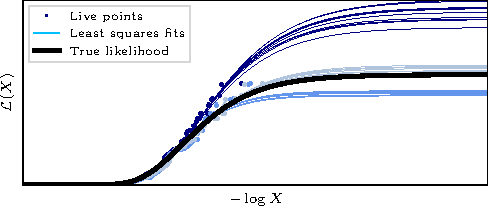
\includegraphics[max width=\linewidth]{figures/prediction_uncertainty.pdf}
\end{center}
\caption{Sources of the prediction uncertainty. The navy points are the live points, plotted for three different instances of $\set{X_i}$ drawn from its distribution. The light blue lines show the uncertainty in the least squares fits over each instance, which is much less than the uncertainty in the spread of the $X$ samples due to long term drift.}
\label{fig:prediction_uncertainty}
\end{figure}

\section{Results}\label{sec:results}
Now that we have a method for predicting the endpoint, we can test it on a range of likelihoods. We shall first present results for cosmological chains in \cref{subsec:cosmological_examples}, for which the method works well. \cref{subsec:toy_examples} will then show some toy examples that are designed to reveal some of the limitations of the method.

\subsection{Gaussians}\label{subsec:gaussians}
We will first test our prediction model on truly Gaussian likelihoods to show that it is able to recover the true parameters as well as the correct endpoint. Let us begin with a spherically symmetrical Gaussian which matches the form of the fitting function, which we can use to check that the correct parameters are inferred when the model is exact. We fix the parameters $\log\mathcal{L}_\mathrm{max} = 0$ and $\sigma = 0.01$ and vary the dimension to see the impact on the predictions.
\par
The inferred parameters are shown in \cref{fig:gauss_params}. The uncertainty in $d$ and $\sigma$ remain large throughout the run, but the endpoint predictions converge because we have already accumulated most of the evidence.
\par
\begin{figure*}
\begin{center}
	\includegraphics{figures/gauss_params.pdf}
\end{center}
\caption{Parameter inferences for the Gaussian fitting function in the $d=8$ case. The true parameters fall within the standard error bars for practically every point, as seen in comparison to the true parameter values shown in the dotted red. The uncertainties remain relatively constant for $d$ and $\sigma$, but the endpoint predictions converge because we have already accumulated most of the evidence.}
\label{fig:gauss_params}
\end{figure*}
Predictions are shown in \cref{fig:gauss_predictions}, where the x-axis plots the negative log-compression as a measure of the progress, so that the run proceeds in the rightward direction. The y-axis shows the predicted log-compression $\log\hat{X}_\mathrm{f}$ at which the termination condition is met.
\par
The true endpoint is recovered to within $2\sigma$ for all runs, but the uncertainty is greater for the higher dimension and $\DKL$ likelihoods. This reflects the fact that the live points typically probe only $\sim \log n_\mathrm{live}$ away from the current dead point. For larger $\DKL$ therefore, the set of samples at any given iteration before the end are quite far from the posterior bulk, and hence poorly resemble the shape of the true posterior.

\subsubsection{Elongated Gaussian}
Consider same example as that presented in \cref{sec:constrained_parameters}. The predictions are initially awry because samples from three of the parameters are uniform. Cannot determine whether these parameters are unconstrained or simply high variance at the midway point. So the predictions are fundamentally limited by the information contained in the samples, not by the prediction method.  

\subsubsection*{Comparison to extrapolating evidence increments}
Seasoned users of nested sampling might be curious how the method compares to simply extrapolating the increments of evidence to roughly estimate when the evidence converges. We do this for a spherical Gaussian as a comparison to our method. At an intermediate stage of the run, the most recent outputs might look something like that shown in the first two columns of the table in \cref{fig:inc_extrapolate}. Extrapolating those data to a linear and exponential profile yields endpoint estimates plotted in the graph to the right. 
\par
The linear extrapolation is clearly an underestimate, since it fails to account for the long tail of the nonlinear profile. The increments are also not quite exponential, since the exponential fit leads to a large overprediction. The predicted endpoint over the course of a run for $d = 16$, $\sigma = 0.01$, as shown in \cref{fig:inc_predictions}, shows the same result. One might expect an average to be more accurate, but this tends to be biased towards the exponential prediction, and there is no obvious choice of weighting that would fix this.
\par
More importantly, we find that for real likelihoods which have an element of noise the extrapolation often diverges, for instance when the increments do not monotonically decrease. Directly extrapolating the evidence increments is therefore far less stable than the previous method, and generally not a reliable method for prediction.
\begin{figure}
\begin{adjustbox}{valign=t, scale=0.72}
\subfloat{\begin{tabular}{|c|c|c|}
\hline
iteration & log Z  & $d\log Z$   \\
\hline
5000 & -1435.8 & 190.8 \\
5500 & -1264.6 & 171.2 \\
6000 & -1123.7 & 140.9 \\
6500 & -991.5 & 132.2 \\
7000 & -885.0 & 106.6 \\
7500 & -790.3 & 94.7 \\
8000 & -702.6 & 87.7 \\
8500 & -619.7 & 82.9 \\
9000 & -551.8 & 67.9 \\
9500 & -492.7 & 59.1 \\
\hline
\end{tabular}}
\end{adjustbox}
\quad
\begin{adjustbox}{valign=t}
\subfloat{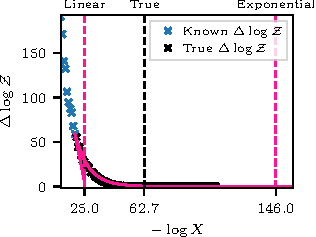
\includegraphics{figures/inc_extrapolate.pdf}}
\end{adjustbox}
\caption{Extrapolating the increments of evidence. The left column shows the output of a nested sampling run, and the right column shows the extrapolation}
\label{fig:inc_extrapolate}
\end{figure}

\begin{figure}
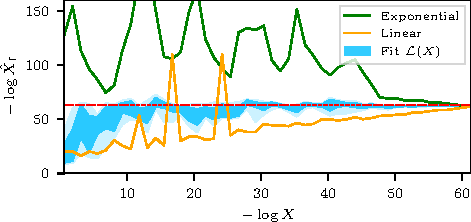
\includegraphics{figures/inc_predictions.pdf}
\caption{Extrapolating the increments of evidence. The left column shows the output of a nested sampling run, and the right column shows the extrapolation}
\label{fig:inc_predictions}
\end{figure}

\subsection{Cosmological examples}\label{subsec:cosmological_examples}
Having established that the prediction framework works for Gaussian likelihoods, we now turn to some cosmological examples, namely chains based on the \textsc{Planck 2018} dataset as described in \citet{curvature_tension}. Predictions are shown in \cref{fig:lcdm_predictions}, with the correct endpoint inferred to within error before the halfway point for all likelihoods.
\par
Most predictions fail to converge at early stages of the run. We find that this is not a consequence of the prediction model, but due to the effective dimensionality of the samples being lower than the true value at the beginning of the run, as was seen in \cref{sec:current_temperature}.

\subsubsection*{Compressive phase transitions}
\begin{figure}
\begin{center}
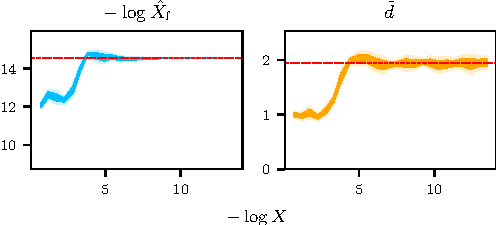
\includegraphics{figures/phase_transition.pdf}
\end{center}
\caption{Endpoint predictions and effective dimensionality as a function of compression for a two-dimensional Gaussian in a box prior $\in [0, 1]$. The parameter variances are $10^{-2}$ and $10^{-5}$ respectively, leading to compression only along one direction initially, which is reflected in $\tilde{d}$. The endpoint only converges when the dimensionality does; before that point the samples genuinely suggest that the likelihood is one-dimensional.}
\label{fig:phase_transition}
\end{figure}
The initial dimensionality of the $\mathcal{L}(X)$ curve is so extrapolating from the curve would fail to account for the true dimensionality of the likelihood, giving inaccurate predictions.
\par
The extrapolation now accounts for the true dimensionality, so the predictions become accurate. The trouble is that before this has happened, the samples really do behave as if they are only constrained in a single dimension! It could really be the case that there is no second parameter, and without our extra knowledge there is no way to detect whether there are two, or even three or more unseen parameters hiding at higher compressions
\par
The different rates of compression for different parameters therefore induce an effective phase transition in the number of degrees of freedom. One can put this on a more quantitative footing by considering the \textit{effective dimensionality} of the posterior. Define the Bayesian model dimensionality $\tilde{d}$ as the posterior variance of the information content, which is given by
\par
\cref{fig:phase_transition} plots the effective dimensionality alongside the endpoint predictions, where it is evident that the predictions are directly dependent on $\tilde{d}$. Introducing correlations between the parameters (not shown) causes the transition to be less sharp, since the more constrained parameter is able to `drag' the other parameter with it, allowing the predictions can be converge shortly before the dimensionality.

\subsection{Edge cases}\label{subsec:toy_examples}
In the cosmological cases, underestimated predictions at early stages was due to the difference in parameter compression rates. However, there are also cases where the form of the fitting function causes problems.
\par
One such instance is a spherical Cauchy likelihood. In fact, at early stages direct least squares fitting fails completely by predicting a remaining evidence that overflows. This can be explained by the fact that a long tail of a Cauchy resembles a Gaussian of much higher dimension, and inferring the dimensionality is unstable. Since we have a stable measure of dimension from the Bayesian model dimensionality, a partial fix is to set $d = \tilde{d}$ instead of inferring it, then using \cref{eq:sigma,,eq:logLm} to get $\log\mathcal{L}_\mathrm{max}$ and $\sigma$.
\par
Results are shown in \cref{fig:cauchy_predictions}, where the likelihood has the form
\begin{equation}
	\log\mathcal{L} = \log\mathcal{L}_\mathrm{max} - \frac{1 + d}{2} \log \left(1 + \frac{X^2}{\gamma^2}\right),
\end{equation}
choosing $d = 10$ and allowing $\gamma$ to vary. However, the extrapolations still fall outside fall outside the standard error range despite isotropic compression. The issue in this case is that the Gaussian fitting function is unable to capture the true shape of the likelihood. A more comprehensive fix would be to use a more flexible fitting function that is able to capture a broader family of likelihoods, which is outside the scope of this paper. Nevertheless, the order of magnitude is still accurate, which remains highly useful to the end user. 

\begin{figure*}
\begin{center}
	\subfloat[Predictions for a spherically symmetric Gaussian likelihood. The correct endpoint is ascertained to within standard error from the beginning for all runs, but the uncertainty is larger for the higher dimension and $\DKL$ likelihoods, reflecting the fact that the live points are further away from the posterior bulk in those cases.]{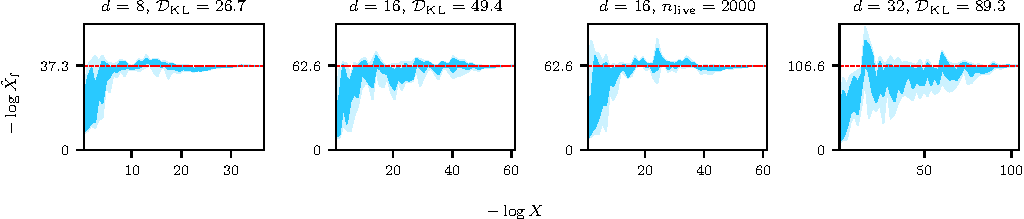
\includegraphics{figures/gauss_predictions.pdf}\label{fig:gauss_predictions}}
	\\[5ex]
	\subfloat[Predictions for the $\Lambda$CDM model. The chains without \textsc{Planck} have low $\DKL$ of below 10, so the live points are relatively close to the posterior bulk at all times and the predictions are quite accurate. ]{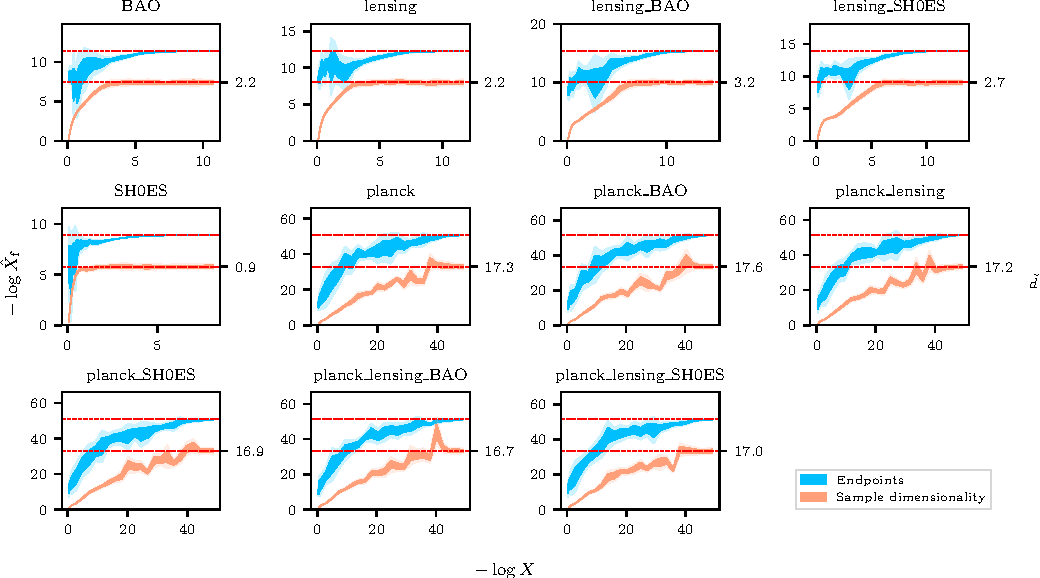
\includegraphics{figures/lcdm_predictions.pdf}\label{fig:lcdm_predictions}}
	\\[5ex]
	\subfloat[Predictions for a Cauchy likelihood. The parameters of the fitting function are obtained by fixing $d = \tilde{d}$, then least squares optimising $\log\mathcal{L}_\mathrm{max}$ and $\sigma$.]{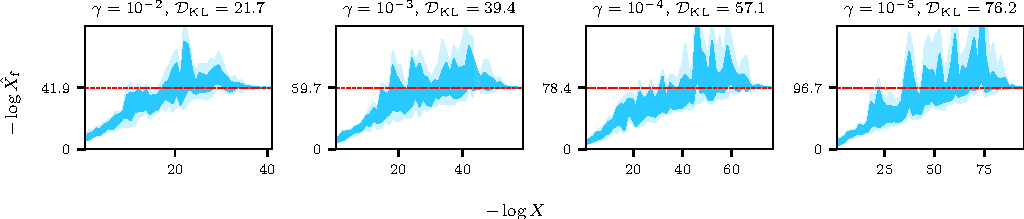
\includegraphics{figures/cauchy_predictions.pdf}\label{fig:cauchy_predictions}}
\end{center}
\caption{Endpoint predictions for different likelihoods. The x-axis shows the negative log-compression, and the y-axis the predicted endpoint $\log\hat{X}_\mathrm{f}$. The shaded regions show the 1 and 2$\sigma$ uncertainties, while the red dashed line shows the true value.} 
\end{figure*}

\section{Conclusions}\label{sec:conclusions}
We have presented a method for predicting the endpoint of a nested sampling run, based on extrapolating the known likelihood profile into higher likelihood regions using a Gaussian fitting function.
\par
The method in general converges to the correct endpoint by about the halfway point, and gets the correct order of magnitude throughout. Predictions are poor when the effective dimension of the samples is lower than the true posterior, but this is a limitation of the information content in the samples rather than our method.
\par
Further work can be done to incorporate more flexible fitting functions to extrapolate non-Gaussian likelihoods, as well as developing a more rigorous framework to choose between the inferred $d$ and $\tilde{d}$.

\bibliographystyle{mnras}
\bibliography{references}

\appendix
\section{Derivation of the termination log-likelihood }
Assume a Gaussian likelihood
\begin{equation}\label{eq:logL}
	\log\mathcal{L} = \log\mathcal{L}_\mathrm{max} - \frac{X^{2/d}}{2\sigma^2}.
\end{equation}
The distribution of the true posterior in $\log\mathcal{L}$ is
\begin{equation}
    P(\log\mathcal{L}) = \frac{1}{\Gamma(\frac{d}{2})}e^{\log\mathcal{L}-\log\mathcal{L}_\mathrm{max}} (\log\mathcal{L}_\mathrm{max}-\log\mathcal{L})^{\frac{d}{2}-1}
\end{equation}
i.e. $2(\log\mathcal{L}_\mathrm{max}-\log\mathcal{L}) \sim \chi^2_{d}$, which is the distribution of the weighted samples. The posterior average and variance of $\log \mathcal{L}$ are given by
\begin{equation}
    \langle\log\mathcal{L}\rangle_\mathcal{P} = \log\mathcal{L}_\mathrm{max} - \frac{d}{2},  \quad \mathrm{Var}(\log\mathcal{L})_\mathcal{P} = \frac{d}{2}.
\end{equation}
Meanwhile, the live points are uniformly distributed over the constrained prior and hence have probability distribution
\begin{equation}
	P(\log\mathcal{L}) = \frac{d}{2}\frac{(\log\mathcal{L}_\mathrm{max}-\log\mathcal{L})^{\frac{d}{2}-1}}{(\log\mathcal{L}_\mathrm{max}-\log\mathcal{L}_*)^{\frac{d}{2}}} \quad [\log\mathcal{L}_* < \log\mathcal{L} <\log\mathcal{L}_\mathrm{max}],
    \label{eq:PL}
\end{equation}
It is helpful at this stage to define a parameter
\begin{equation}
    y = \frac{\log\mathcal{L}-\log\mathcal{L}_*}{\log\mathcal{L}_\mathrm{max}-\log\mathcal{L}_*}
    \label{eq:y}
\end{equation}
as a normalised measure of how far a point is between the latest dead point and the maximum log-likelihood, with $y=0$ corresponding to $\mathcal{L}_*$ and $y=1$ to $\mathcal{L}_\mathrm{max}$, so that
\begin{equation}
    P(y) = \frac{d}{2}(1-y)^{\frac{d}{2}-1} \quad [0<y<1].
    \label{eq:Py}
\end{equation}
We now seek the distribution for the maximum likelihood of the live points, $\log\mathcal{L}_\mathrm{max}^{\mathrm{live}}$. Using the result that the maximum of $n$ variables with cumulative distribution $F(y)$ follows $\frac{d}{dy}( 1- (1-F(y))^n)$, we obtain
\begin{equation}
    P(y_\mathrm{max}^\mathrm{live}) = \frac{nd}{2}(1-y_\mathrm{max}^\mathrm{live})^{\frac{d}{2}-1}\left(1-(1-y_\mathrm{max}^\mathrm{live})^{\frac{d}{2}}\right)^{n-1}[0<y_\mathrm{max}^\mathrm{live}<1],
    \label{eq:Pyhat}
\end{equation}
which in the limit of large live points and dimensions can be roughly summarised by
\begin{equation}\label{eq:ylivemax}
	    \lim_{d,n\to\infty} y_\mathrm{max}^\mathrm{live} \sim \frac{2\log n}{d} \pm \sqrt{\frac{2}{3}}\frac{\pi}{d}.
\end{equation}
This shows that in general the live points are nowhere near the maximum log-likelihood at any iteration, though they do steadily squeeze the interval $[\log\mathcal{L}_*,\log\mathcal{L}_\mathrm{max}]$. In particular, in high dimensions $n$ only gets us harmonically/logarithmically closer, whilst $d$ pushes us linearly further away.
\par
This remains true even at the end of the nested sampling run. To see this, we write the halting condition as:
\begin{equation}
	f = \frac{\int_0^{X_\mathrm{end}} \mathcal{L}\ \mathrm{d}X}{\int_0^\infty \mathcal{L}\ \mathrm{d}X}.
    \label{eq:fint}
\end{equation}
Note that we have assumed that prior effects are negligible (so $1=\infty$), and that $f \ll 1$ so that the denominator is approximately the accumulated evidence. Computing this for \cref{eq:logL} we find the answer in terms of lower incomplete gamma functions
\begin{equation}
    f = 1- \frac{\Gamma_{d/2}\left(\frac{X_\mathrm{end}^{2/d}}{2\sigma^2}\right)}{\Gamma\left(\frac{d}{2}\right)}.
    \label{eq:f}
\end{equation}
Taking the $X_\mathrm{end}\ll (\sqrt{2}\sigma)^d$ limit (almost certainly valid at termination) we find
\begin{equation}
    \lim_{X_\mathrm{end}\ll (\sqrt{2}\sigma)^d} f \approx \frac{X_\mathrm{end}}{(\sqrt{2}\sigma)^d \ \Gamma(1+\frac{d}{2})} = \frac{(\log\mathcal{L}_\mathrm{max}-\log\mathcal{L}_\mathrm{end})^{\frac{d}{2}}}{\Gamma(1+\frac{d}{2})}.
\end{equation}
We thus have an expression relating $\mathcal{L}_\mathrm{end}$ at termination to the termination fraction $f$. This becomes yet more pleasing in the large $d$ limit, since $f^{2/d}\to 1$, we find via a Stirling approximation:
\begin{equation}
    \lim_{d\to\infty} \log\mathcal{L}_\mathrm{end} \approx \log\mathcal{L}_\mathrm{max} - \frac{d}{2e}.
\end{equation}
In the event that we keep $f$ in, we replace $\frac{d}{2e}\to \frac{d}{2e}f^{2/d}$, so we can of course battle the $\frac{d}{2e}$ term, but this becomes exponentially difficult in high dimensions.
\par
Putting this together, taking $\mathcal{L}_*$ in \cref{eq:y} to be $\mathcal{L}_\mathrm{end}$, and combining this with \cref{eq:ylivemax} we find
\begin{equation}
    \boxed{
        \log{\mathcal{L}}_\mathrm{max}^\mathrm{live} \approx \log\mathcal{L}_\mathrm{max} - \frac{d}{2e} + \frac{\log n}{e} \pm \frac{\pi}{\sqrt{6}e}
    },
\end{equation}
showing that in general nested sampling will finish at a contour $d/2e$ away from the maximum log-likelihood, and the final set of $n$ live points can get you $\log (n)/2e$ closer, with a chance of getting $\sim\pi/\sqrt{6}e=0.472$ closer still by statistical fluctuation. This general anatomy is shown in \cref{fig:anatomy}.

\label{lastpage}
\end{document}

